\documentclass[a4paper, 11pt]{article}
\usepackage[utf8]{inputenc}

\usepackage[a4paper]{geometry}
\usepackage{graphicx}
\usepackage{listings}
\usepackage{color}
\usepackage{amsmath}
\newcommand\norm[1]{\left\lVert#1\right\rVert}
\usepackage{amsfonts}
\usepackage{float}
\usepackage{tabularx}
\usepackage{url}


\newcommand{\HRule}{\rule{\linewidth}{0.5mm}}

\title{Authentication at scale}
\author{ }
\date{Spring 2015}

\begin{document}

\newgeometry{top=3cm, bottom=3cm, left=2.5cm, right=2.5cm}

\begin{titlepage}
\begin{center}

\begin{figure}[h] 
\begin{center}
\begin{minipage}[c]{.45\linewidth}
\begin{center}

\includegraphics[scale=1]{images/logoEPFL.png}
\end{center}
\end{minipage}
\end{center}
\end{figure}

\hfill \\[2cm]
\HRule \\[0.5cm]
{ \Huge \bfseries Event Stream Detection}\\[0.5cm]

\HRule \\[2cm]
\makeatletter
\renewcommand{\thesection}{\@arabic\c@section}
\makeatother
\textsc{\textbf{\Large BigData2015 - CS422\\ Digital Humanities Laboratory}}\\[2cm]


\large Laurent \textsc{ANADON}\\
\large Antoine \textsc{BASTIEN}\\
\large Antoine \textsc{BODIN}\\
\large Matias \textsc{CERCHIERINI}\\
\large Nina \textsc{DESNICA}\\
\large Louis \textsc{FAUCON}\\
\large Damien \textsc{HILLOULIN}\\
\large Christian \textsc{MOUCHET}\\
\large Sami \textsc{PERRIN}\\[2cm]


\begin{tabular}{rl}
\textsc{Professor:} &\textsc{Christoph KOCH}\\
\textsc{Teaching Assistant} &\textsc{Immanuel TRUMMER}\\
\textsc{DHLab Supervisor} &\textsc{Yannick ROCHAT}
\end{tabular}

\hfill \\[1cm]
{\large Spring 2015}
\end{center}
\end{titlepage}

\restoregeometry
\tableofcontents
\newpage


\section{Introduction}
\paragraph{}
Along with the 2015 Big Data course, we are leading a project addressing topic detection in news streams for the DHLab\footnote{Digital Humanities Laboratory} as part of a course project. We aim at detecting articles that talk about the same topic over a set of issues contiguous in time, and across two newspapers over more than 150 years:
\begin{itemize}
\item \emph{Journal de Genève} (JDG) from 1840 to 1998,
\item \emph{Gazette de Lausanne} (GDL, under different names) from 1840 to 1998.
\end{itemize}
To do this, we are looking into clustering, hierarchical clustering and correlations detection techniques. One of the main challenges here is the huge amount of data: we are considering articles over a huge time span, which is why we need the algorithms we implement to be scalable.

\paragraph{}
In order to achieve this goal, we focus upon previous studies such as \cite{kdd05-ttm} and try to use this in the context of the big data and the requirements of Spark.
First of all, we parse articles and store them inside convenient distributed data structures through Spark RDDs, and secondly we extract releveant themes among articles over a well choosen time period with parallelized machine learning algorithms. Once this is done, we find correlations between these themes to build the evolutionary graph. Eventually, we analyze the life cycles of themes and measure their strength over time.

\newpage

\section{Description of the algorithm}

\section{Data Modeling and Article Extraction}
The first phase in the program consists in parsing the article streams and producing the data structures needed in the subsequent steps. Though conceptually simple, the parsing has been challenged by several practical constraints. We will first give an overview of the data generated in this phase, and then a more technical description of the processing steps. Lastly, we will describe the practical problems we encountered and how we dealt with them.

\subsection{Data description}
The dataset is a collection of 159 years worth of articles for the \emph{Gazette de Lausanne} and 156 for the \emph{Journal de Genève}. The period starts from 1840 and ends in 1998 for both newspapers. The format of the data is a one-liner XML file per year and per newspaper. The root node contains one \textit{article} node per article, themselves containing one or several \textit{entities} per article part (if the article spans over multiple pages, for example). Each entity contains the associated article in plain text and all the metadata related to the article. The ones we used for our application were the \textit{issue date}, \textit{page number}, \textit{title} and \textit{publication}. The plain text is the result of an OCR scan of the original newspaper archive. Consequently, it is very noisy and contains lots of character recognition mistakes.
The total size of the dataset is 7.1 Go and 9.6 Go for the \emph{Gazette de Lausanne} and \emph{Journal de Genève} collections respectively.

\subsection{Parser output overview}
During such a long period, the French language has been subject to a progressive drift. In a way, the streams are composed of slightly different idioms which belong to particular temporal slices. Typically, a word like "Internet" only appears in the later part of the streams. In our project, this could potentially create a bias because of the background model, a structure described below. In order to compensate this, the program will not analyze the entire dataset, but a temporal subset which we define as the \emph{time frame}. Consequently, from the program's "perspective", the time frame acts as the dataset, so we will use this term instead when there is no ambiguity.
The \emph{background model} is an unique object on the whole dataset (i.e time frame). It allows to retrieve the distribution of every distinct word in the dataset. This structure is used during the theme analysis to determine how common a word is. At the time we needed to fine-tune our algorithms, it came out that having a \emph{background model} on a larger temporal subset than the time frame could improve results. Therefore, we defined a new time period type called  \emph{background model time frame}.
For the next part, we will differentiate two different phases in the processing pipeline: the theme extraction, where we perform the Expectation-Maximization (EM) algorithm, and the theme "strength" analysis, which uses the Hidden Markov Models (HMM). Both phases are described later. For the EM phase, the parser has to provide a structure containing the word count inside each individual article text. For that, we use an object representing a \emph{parsed article}, which contains the count of each distinct word in this article, as well as some other properties (issue date, stream identifier...). These parsed articles must be grouped by small sub-partitions of the time frame that we called \emph{time partition}s. Effectively, the EM part receives an RDD of \emph{time partition}s containing a small part of the parsed articles. The HMM part requires the chronological concatenation of all the words in the \emph{time frame} , where a timestamp is attributed to each word. In order to reduce the memory and CPU usage of such a structure, we don't store the words as Java String objects; rather, we first associate each distinct word to a unique integer identifier, and then produce the word concatenation as an ordered RDD of integers. Both the EM and HMM parts need to access the background model. Figure \ref{fig:time_entities} summarizes the different time entities we defined.

\begin{figure}
   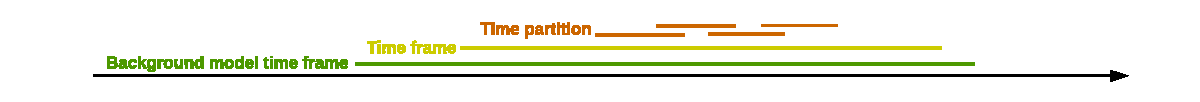
\includegraphics[width=\textwidth]{time_entities.pdf}
   \caption{\label{fig:time_entities} The different types of time periods on a time-line.}
\end{figure}

\subsection{Data processing pipeline}
The parser does not produce all its output on a single method call. The background model must be computed at the beginning, but the input provided for the EM and HMM parts are generated "on demand", in order to avoid storing pending data (we don't want to keep the HMM input for the whole execution, only to use it once at the end). However, it would be expensive to parse and transform the XML files from scratch at each of these steps. Instead, we produce an intermediary RDD from which all these outputs can be derived. First, we parse the XML streams, retrieve the articles, and segment their text content into a list of words. This list, along with other information about the article like the issue date and the title, are stored in a container we named \emph{segmented article}, which is accumulated in our base RDD.
The background model is generated immediately after this base RDD is computed.
We generate the EM phase input on demand by associating each word to its number of occurrences inside every segmented article individually. Using a provided partitioning of the \emph{time frame} into \emph{time partitions}, the parser returns the RDD of grouped parsed articles.
Finally, for the HMM phase, we first use the background model to build a lexicon that translates each unique word into an integer identifier. The segmented articles are then sorted chronologically, after what we extract their lists of words, translate them into lists of identifiers using the lexicon, and assemble all the results in one single RDD. This is done on demand by a method call at the time we run the HMM phase.
It is noticeable that some of these operations are quite redundant. Part of this problem is due to the fact that we are exposed to a "chicken-and-egg" situation; the background model must be produced from the list of extracted articles, but we also need the background model during the processing of the article RDDs (and not only for the HMM phase as we will see in the next section). Because of this, and other optimizations that we describe below, we inevitably apply similar transformations over the whole dataset. Nevertheless, all of the operations are particularly simple and can be fully parallelized, resulting in a satisfying total execution time.

\begin{figure}
   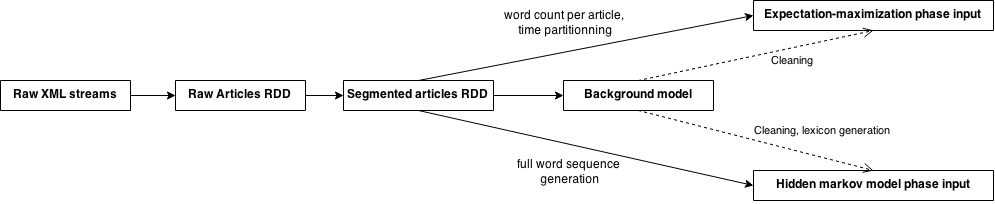
\includegraphics[width=\textwidth]{parser_processing_steps.png}
   \caption{\label{fig:parser_processing_steps} Parser processing pipeline}
\end{figure}

\subsection{Data cleaning and filtering}
The parser also enable some basic cleaning and filtering functionality. There was two main factor for noise introduction: OCR errors and meaningless (for us) articles. The problem with OCR errors is that they make the size of the \emph{background model} grow linearly with the \emph{background model time frame} length because of the "new" words they introduce. This is a problem because the \emph{background model} needs to fit in main memory and is queried very frequently. The adopted solution is to set a threshold on the word frequency. Word above the given frequency are simply discarded from the articles and the \emph{background model}. This way, unusual OCR error are discarded, while the usual ones are part of the \emph{background model} so that they do not disturb later stages.
To address the meaningless articles problem, we can set two parameters at parse time. The first is a threshold on the number of word per article. Articles having count above this threshold are discarded. The second is the page number threshold. It filters out article that begins at page greater than the threshold. The problem with this is: it is not always the case that article on the first pages are the most relevant ones as we are used to.
In fact, setting those parameters is very tricky and depends on the \emph{time frame} of interest. Better understanding of written press at this time is in fact needed to accomplish this.


\section{Theme Extraction}
\label{sec:themeExtraction}

\paragraph{}
Once the data is extracted by the parser, the first task we need to tackle is to detect themes in the data collection. This is also known as topics clustering and is done by performing soft clustering on the words probability distributions.

\paragraph{}
Because of the very large time span of the collection, detecting a precise theme over the entire collection is almost impossible. To overcome this issue, the method in \cite{kdd05-ttm} splits the collection into several sub-collections $C_{i}$ (that we name \emph{time partition}) where the themes are extracted independently from each other.

\subsection{Probabilistic Model}

\paragraph{}
Themes are extracted from every time partition $C_{i}$ using a probabilistic mixture model and the expectation-maximization algorithm where the themes are the parameters to estimate. The latent variables of this model are k themes  $\theta_{1}$,...,$\theta_{k}$ and a background model $\theta_{B}$ for the whole collection. The presence of the background model variable is justified by the need to remove non-discriminating and non-informative words to describe a theme. The proportion of the background model is regulated by the mixing weight $\lambda_{B}$.

\paragraph{}
The goal of the algorithm is to maximize the following log-likelihood in a model:

\begin{center}

$
\sum_{d\in C_{i}} \sum_{w} [c(w,d)log(\lambda_{B}p(w|\theta_{B}) + (1-\lambda_{B})\sum_{j=1}^{k} (\pi_{d,j} p(w|\theta_{j})))]  
$

\end{center}

where 

\begin{itemize}
\item c(w,d) is the count of word w in document d
\item $p(w|\theta_{j})$ is the probability of having the word w in the theme j, knowing the theme distribution $\theta_{j}$
\item $p(w|\theta_{B})$ is the probability of having w in the background model, knowing $\theta_{B}$
\item $\pi_{d,j}$ is the probability that document d belongs to theme j
\end{itemize}

\paragraph{}
By initializing the $p(w|\theta_{j})$ randomly and the $\pi_{d,j}$ uniformly, we can perform several iterations of the expectation-maximization algorithm in order to maximize the log-likelihood. One iteration is given by the following formulas to update the latent probabilities:

\begin{equation*}
p(z_{d,w} = j) = \frac{\pi_{d,j}p(w|\theta_{j})} {\sum_{j\prime=1}^{k} {\pi_{d,j\prime}p(w|\theta_{j\prime})} }
\end{equation*}

\begin{equation*}
p(z_{d,w} = B) = \frac
{\lambda_{B} p(w|\theta_{B})} 
{\lambda_{B} p(w|\theta_{B}) + (1-\lambda_{B})
\sum_{j\prime=1}^{k} {\pi_{d,j\prime}p(w|\theta_{j\prime})}}
\end{equation*}

\begin{equation*}
\pi_{d,j} = \frac
{\sum_{w}{c(w,d)(1-p(z_{d,w} = B))(p(z_{d,w} = j))}}
{\sum_{j\prime=1}^{k}{\sum_{w}{c(w,d)(1-p(z_{d,w} = B))(p(z_{d,w} = j\prime))}}}
\end{equation*}

\begin{equation*}
p(w|\theta_{j}) = \frac
{\sum_{d\in C_{i}}{c(w,d)(1-p(z_{d,w} = B))(p(z_{d,w} = j))}}
{\sum_{w\prime}{
\sum_{d \in C_{i}} {c(w\prime,d)(1-p(z_{d,w\prime} = B))(p(z_{d,w\prime} = j))}}}
\end{equation*}


\paragraph{}
Because the convergence of the EM algorithm is not guaranteed, we need to run several times the algorithm with different initial probabilities.

\paragraph{}
The same model is applied to every sub-collection independently from each other. Only the background model is common but it is not updated during the iterations of the EM algorithm. 

\paragraph{}
Finally, we compute for each theme the average probability that documents belong to this theme. This enables us to filter some of them out for future steps.

\subsection{Implementation with Spark}

\paragraph{}
The fact of having multiple time partitions dividing the whole collection of articles is well suited for parallelization. Indeed, for each time partition (class EmInput), we process one expectation-maximization algorithm to its articles. There are no dependencies between different time partitions during the execution of the algorithm.

\paragraph{}
The class EmAlgo clones every EmInputs depending on the number of trials we choose and launch the EM algorithm concurrently. All iterations of one EmInput are performed within one map function to avoid time losses between executors or re-computations if Spark drops an output. Then, EmAlgo chooses the EmInput object that has the highest log-likelihood for each time period.

\paragraph{}
By testing our implementation with different parameters, we could see that it gives nice results with a mixing weight of the background model around 0.92. A higher value removes very important words (such as "war" in war time) and a lower value adds a lot of verbs to the results ; contrary to English, in French the informative words are mostly nouns not verbs.

\subsection{Complexity}

\paragraph{}
Once all the articles are parsed and the time partitions generated, the complexity and computation time of the expectation-maximization algorithm depend mainly on the number of articles, the number of themes and the number of iterations of the EM algorithm.
The size of the background model has also a non-negligible influence as the algorithm is going through the map multiple times at each iteration. However, this size doesn't grow linearly with the number of articles and we can clean words from every set of probabilities if the appearance doesn't exceed a minimum threshold.

\paragraph{}
In order to maintain efficient scalability, we choose a period defining the time partition of one week. The choice of this time period is a good trade-off as it is precise enough to locate events and enables us to have enough articles in each time period. Indeed, it gives us between 100 and 200 articles in each time partition to process which take about one minute to extract 10 themes.

\subsection{Results}

\paragraph{}
After running the expectation-maximization algorithm on specified time periods, we could extract relevant themes. We could observe that if there was no clear event at this time, it was not always easy to guess the meaning of the dectected theme, sometimes because it referred to precise events unknown from us, and sometimes because it was only consisting of noise. Fortunately, most of these themes can be filtered out based on their score. Some other themes provided real clear descriptions and we could easily know to which event the theme was referring.

Here are some example of relevant themes at the beginning of World War I in 1914:

\begin{center}
\begin{tabular}{|l|l|l|}
  \hline
  Jul 26 - Aug 3 & Aug 3 - Aug 10 & Aug 10 - Aug 17 \\
  \hline
  juillet & allemagne & allemands \\
  berlin & france & troupes \\
  mobilisation & frontière & guerre \\
  situation & mobilisation & français \\
  vienne & guerre & allemandes \\
  belgrade & français & ambassadeur \\
  guerre & luxembourg & pétersbourg \\
  russie & neutralité & bruxelles \\
  \hline
\end{tabular}
\end{center}

\paragraph{}
In addition, when the vocabular changes a lot in some set of articles, themes are well descripted. Here is a theme describing the first landing on the moon which was huge event and a theme describing the Panama Treaty in 1978, which was less covered by the press.


\begin{center}
\begin{tabular}{|l|l|}
  \hline
  Jul 17 - Jul 24 1969 & Jan 29 - Feb 5 1978 \\
  \hline
  apollo & panama \\
  lunaire & traités \\
  armstrong & ratification \\
  houston & frolinat \\
  aldrin & rebelles \\
  espace & carter \\
  \hline
\end{tabular}
\end{center}




\subsection{Evolution Graph}
\paragraph{}
In section \ref{sec:ThemeExtraction} we showed a method to extract themes from the dataset of articles over a given period of time. However we are interested in detecting events that can last for a long time. This is why we studied evolutionary transitions. In section \ref{sec:EvoGraphInterest} we introduce the Kullback divergence which allow to measure the distance between extracted themes and we show how it can be interpreted to detect long lasting events. Then, in section \ref{sec:EvoGraphImplementation} and \ref{sec:EvoGraphPerformance}, we present our implementation in parallel using spark and its performance. Finally in section \ref{sec:EvoGraphResults} we show the results obtained by this method.

\subsubsection{Interest}
\label{sec:EvoGraphInterest}

\paragraph{}
Since themes are basically probability distributions of words over a given time period, in [citation needed], they recommend to use the Kullback divergence which is commonly used in information theory to compare communication channels [citation needed] :\[ D(Theme1 || Theme2) = \sum_{word} P(word|Theme1) log(\frac{P(word|Theme1)}{P(word|Theme2)})\]where $P(word|theme)$ is the probability of reading the word $word$ in an article if it deals with the theme $theme$. Here we use it to have a measure of the difference between the probability distributions of two themes. An other solution to compare probability distributions is to use the Total Variation distance [citation needed] :\[ \norm{Theme1 - Theme2}_{TV} = \frac{1}{2} \sum_{word} |P(word|Theme1) - P(word|Theme2)|\]We implemented both solution and as expected the...

\paragraph{}
With this distance, we now consider that there is an evolutionary transition between two themes, $T_1$ and $T_2$, if $T_2$ comes after $T_1$ in the time-line and if the divergence is bellow a threshold that we choose. This way we build the evolution graph with themes as vertices and evolutionary transition as edges. Paths in this graph will reflect how a given theme is slightly transformed from one period of time to an other. We will then be able to see both the real length of an event in time and also if new elements appeared at some point. [example needed]

\subsubsection{Implementation}
\label{sec:EvoGraphImplementation}
\paragraph{}
The implementation works like ...

\paragraph{}
We used smoothed probabilities as it is discussed in \cite{de2010grammatical} because ... 

\subsubsection{Performance}
\label{sec:EvoGraphPerformance}
\paragraph{}
Even so we parallelize the work efficiently, the evolution graph algorithm does not fit the definition of scalable. Indeed, if we have twice as many periods of time and twice as many executors the running time does not stay the same. It will be in fact multiplied by two. This is due to the inherent quadratic complexity of the algorithm which requires to measure the distance for each pair of themes.

\paragraph{}
We could avoid this quadratic complexity by looking only at similarity between theme that are close to each other in time. However we thought this simplification would make us lose interesting links like for example [pertinent example needed]

\paragraph{}
Our parallel implementation performs well :
\newline
\begin{tabular}{llll}
Number of Theme & Number of pairs & Number of executors & Execution time \\
\~ 200 & \~ 20000 & 500 & \~ 10s \\
\~ 2000 & \~ 2000000 & 500 & \~ 7min34s \\
\end{tabular}
\newline
[performance measure to be completed soon]


\subsubsection{Results}
\label{sec:EvoGraphResults}

\paragraph{}
In order to get a graphical representation of the results, we have decided to use GraphViz to generate a graph. Using Spark and the previously generated evolution graph RDD, we have implemented a .dot file generator to build the graph on a particular time-span.
[Graph Exemple Required]


\subsection{Evaluate Themes Strength over time using Hidden Markov Models}
The previous approach was detecting topics in short time periods and expliciting relations between them. Here, we consider the recurrent topics that would happen several times in the whole study period or would last numerous time periods. For this themes, the goal is to be able to determine how the importance of a theme is varying over time.

\subsubsection{Overall Method}
To be able to perform the themes strength analysis, the themes first need to be detected. These themes are \emph{trans-collection themes}. The most straightforward way to find them would be to perform themes detection over very long durations (several years or decades), but the performance of the EM algorithm does not allow that. Indeed, the EM algorithm is well parallelized and efficient when processing many short time periods but a single long window of time would be analyzed sequentially which would require a huge amount of time. Two work-around strategies have been found for this issue :
\begin{itemize}
\item perform the analysis over several shorter time periods and retain only the themes that have the highest probability. Then try to analyse if some of them last longer than other or are recurrent in time.
\item perform the two steps  : EM algorithm and evolutionnary transitions computation. This will leave us with a graph of temporal dependencies between themes. Then the trans-collection themes can be identified as the longest connex components -to be checked!!- in our graph. This allows us to detect the themes that last long or that are recurrent. Finally to obtain the trans-collection themes, the probabilities of the short themes are averaged.

We need a picture here! 

\end{itemize}

\subsubsection{Parallel Baum-Welch Algorithm}
The Baum-Welch algorithm is a classic algorithm to train a Hidden Markov Model given an observed sequence. The algorithm is capable of estimating the initial probability distribution, the transition probability distribution, and the emission probability distribution.
In its most-basic (but efficient) forward-backward version as presented in \cite{rabiner1989tutorial} for example, the algorithm computes some probabilities from the beginning of the observed sequence to the end, and some other probabilities from the end of the observed sequence to the beginning. It has the advantage to be fast compared to other algorithms like the forward only or backward only presented in [ CITATION HERE ] but uses a lot of memory, and is sequential by nature.
Some work has to be done to make it parallel on the observed sequence (as presented for example in [CITATION HERE]), or precise ( as presented for example in [CITATION HERE]). However it seems like no paper presented a variant being precise, and also accelerated in parallel over the observed sequence.
Thus, we extended the known algorithms to design a precise and parallel algorithm for very long observation sequences.
Our algorithm enabled us to train our Hidden Markov Model over a sequence of more than 5 billion observations on a cluster of thousands of processors using Spark. It uses more memory than the original forward-backward version and also makes more computations, but can be run on as many cores as available (as long as there are less processors than observations...).
We will present in the rest of this section the original forward-backward algorithm, the precise variant, and our precise parallel algorithm.

In all the rest of this section, we use the same notations and definitions as on the Wikipedia (English) article of the Baum-Welch algorithm. We first present the original algorithm as on the Wikipedia article, then present the precise version suggested in [RABINER CITATION HERE], then the parallel version suggested in [TURIN, WILLIAM CITATION HERE], and ultimately our precise parallel version which is built upon the two ideas.

\paragraph{Hidden Markov Model}
(This section is a mere copy of the wikipedia article).
Let $X_t$ be the hidden variables (each taking $N$ possible values) and $Y_t$ the observation variables (each taking $M$ possible values). We assume that the Markov chain is homogeneous, that is $P(X_t|X_{t-1})$ is independent from the time $t$.
It is therefore possible to define the transition probability matrix $A = \{a_{i,j}\} = P(X_t = j | X_{t-1} = i)$.
We can define the initial probability distribution as $\pi_i = P(X_1=i)$ and the emission probabilities as $b_j(y_t) = P(Y_t = y_t | X_t = j)$. Usually is defined the emission probability matrix $B = \{b_j(y_i)\} = P(Y_i=y_i | X_j)$.

With such definitions, we can define the parameters of a Hidden Markov Model as the triplet $\Theta = (A, B, \pi)$, where $A$ is the transition probability matrix, $B$ is the emission probability matrix, and $\pi$ is the initial probability distribution.
\paragraph{Baum-Welch Algorithm}
(This section is a mere copy of the wikipedia article).
The Baum-Welch algorithm is an algorithm using the Expectation-Maximization principle to find the parameters $\Theta^*$ such that $P(Y_1,...,Y_T| \Theta^* )$ is a local maximum.
In its forward-backward version,it is necessary to compute first during the forward procedure the coefficients $\alpha_i(t) = P(Y_1=y_1,...,Y_t = y_t, X_t = i | \Theta )$ and then it is necessary to compute the coefficients $\beta_i(t) = P(Y_{t+1}=y_{t+1},...,Y_T = y_T| X_t = i, \Theta )$.

Once those forward and backward coefficients are computed, it is possible to update the initial distribution, transition probability matrix and the emission matries, as shown in [RABINER CITATION HERE] or [WIKIPEDIA ARTICLE HERE].

We have used this forward-backward algorithm as the starting point of our algorithm.
\paragraph{Precise Froward-Backward algorithm}
The original Baum-Welch algorithm depicted in the previous section suffers from precision problems (underflows) when the size of the sequence size grows up.
As presented in [RABINER CITATION HERE], one way to fix that is by defining a family of scaled coefficients $\hat{\alpha}_i(t)$ and $\hat{\beta}_i(t)$ defined by the relations:
\begin{equation}
\begin{cases}
\bar{\alpha}_i(1) = \pi_i b_i(y_1) & \\
\bar{\alpha}_i(t) = b_i(y_t)\sum_{j=1}^{N}{a_{j,i}\bar{\alpha}_j(t-1)} & \text{for t \textgreater 1} \\
c_t = \frac{1}{\sum^N_{j=1} \bar{\alpha}_j(t)} & \\
\hat{\alpha}_i(t) = c_t \bar{\alpha}_i(t) & \text{for all t}
\end{cases}
\end{equation}

And
\begin{equation}
\begin{cases}
\bar{\beta}_i(T) = 1 & \\
\bar{\beta}_i(t) = b_j(y_{t+1})\sum_{j=1}^{N}{a_{i,j}\hat{\beta}_j(t+1)} & \text{for t \textless T} \\
\hat{\beta}_i(t) = c_t \bar{\beta}_i(t)
\end{cases}
\end{equation}

The new update rules are described in [RABINER CITATION HERE].

\paragraph{Precise parallel Forward-Backward algorithm}
As described in [TURIN, WILLIAM CITATION HERE], it is possible to design a parallel forward-backward algorithm from the traditional forward-backward algorithm as the relations defining the forward and backward coefficients are linear. However, the way scaling is done in the precise version of algorithm seems to block this. This is not the case, and we show how in this section.

In the previous section, the relations defining the scaled forward coefficients can be in fact reinterpreted as the following relations:
\begin{equation}
\begin{cases}
\bar{\alpha}_i(1) = \pi_i b_i(y_1) & \\
\bar{\alpha}_i(t) = b_i(y_t)\sum_{j=1}^{N}{a_{j,i}\bar{\alpha}_j(t-1)} & \text{for t \textgreater 1} \\
\hat{\alpha}_i(t) = c_t \bar{\alpha}_i(t) & \text{for all t} \\
\text{with } c_t \text{ such that } \sum_{j=1}^{N}{\hat{\alpha}_j(t)} = 1 & \text{for }t \ge 1
\end{cases}
\end{equation}

While it was previously not possible to design a parallel algorithm due to the definition of the $c_t$ coefficients (hindering the parallel computation of the $\hat{\alpha}_i(t)$ coefficients), it is now possible.
If we define the matrices $\bar{Fo}(t_1 \rightarrow t_1 + 1)$ (one step forward matrices), the matrices $\bar{Ba}( t_1 \leftarrow t_1 + 1)$ (one step backward matrices), the vectors $\bar{\alpha}(t)=(\bar{\alpha}_i(t))$, and the vectors $\bar{\beta}(t)=(\bar{\beta}_i(t))$ with the following relations:

\begin{equation}
\begin{cases}
\bar{Fo}( t - 1 \rightarrow t) =  \{b_i(y_{t+1})a_{ji}\} & \\
\bar{\alpha}(1) =  (\pi_i b_i(y_1))_{1 \le i \le N} & \\
\bar{\alpha}(t) =  \bar{Fo}( t - 1 \rightarrow t) \hat{\alpha}_i(t - 1) & \text{for t \textgreater 1} \\
\hat{\alpha}(t) = c_t \bar{\alpha}(t) &
\end{cases}
\begin{cases}
\bar{Ba}( t \leftarrow t + 1) = \{b_j(y_{t+1})a_{ij}\} & \\
\bar{\beta}(T) = (1)_{1 \le i \le N} & \\
\bar{\beta}(t) =  \bar{Ba}( t \leftarrow t + 1) \hat{\beta}(t + 1) & \text{for t \textless T} \\
\hat{\beta}(t) = c_t \bar{\beta}(t) &
\end{cases}
\end{equation}

It is possible to go parallel with some more general matrices $\bar{Fo}(t_1 \rightarrow t_2)$ (forward matrices), $\bar{Ba}(t_1 \leftarrow t_2)$ (backward matrices), $\hat{Fo}(t_1 \rightarrow t_2)$ (precise forward matrices), $\hat{Ba}(t_1 \leftarrow t_2)$ (precise backward matrices), following these constitutive relations:

\begin{equation}
\begin{cases}
\bar{Fo}( t - 1 \rightarrow t) =  \{b_i(y_{t+1})a_{ji}\} & \\
\bar{Fo}( t_1 \rightarrow t_3) =   \bar{Fo}( t_2 \rightarrow t_3) \hat{Fo}( t_1 \rightarrow t_2)& \\
\hat{Fo}( t_1 \rightarrow t_3) =   \hat{Fo}( t_2 \rightarrow t_3) \hat{Fo}( t_1 \rightarrow t_2)& \\
\bar{\alpha}(t_2) =  \bar{Fo}( t_1 \rightarrow t_2) \hat{\alpha}(t_1) & \\
\hat{\alpha}(t_2) =  \hat{Fo}( t_1 \rightarrow t_2) \hat{\alpha}(t_1) &
\end{cases}
\begin{cases}
\bar{Ba}( t \leftarrow t + 1) = \{b_j(y_{t+1})a_{ij}\} & \\
\bar{Ba}(t_1 \leftarrow t_3) = \bar{Ba}(t_1 \leftarrow t_2) \hat{Ba}(t_2 \leftarrow t_3) & \\
\hat{Ba}(t_1 \leftarrow t_3) = \hat{Ba}(t_1 \leftarrow t_2) \hat{Ba}(t_2 \leftarrow t_3) & \\
\bar{\beta}(t_1) =  \bar{Ba}( t_1 \leftarrow t_2) \hat{\beta}(t_2) & \\
\hat{\beta}(t_1) =  \hat{Ba}( t_1 \leftarrow t_2) \hat{\beta}(t_2) & \\
\end{cases}
\end{equation}

It is possible to go parallel as in fact we can choose any families of matrices $\hat{Fo}(t_1 \rightarrow t_2)$ and $\hat{Ba}(t_1 \leftarrow t_2)$ just guaranteeing that
\begin{equation}
\begin{cases}
\hat{Fo}( t - 1 \rightarrow t) = \frac{\bar{Fo}( t - 1 \rightarrow t)}{\norm{\bar{Fo}( t - 1 \rightarrow t)}_1} & \\
\hat{Fo}( t_1 \rightarrow t_3) =   \frac{\hat{Fo}( t_2 \rightarrow t_3) \hat{Fo}( t_1 \rightarrow t_2)}{\norm{\hat{Fo}( t_2 \rightarrow t_3) \hat{Fo}( t_1 \rightarrow t_2)}_1}& \\
\end{cases}
\begin{cases}
\hat{Ba}(t \leftarrow t+1) = \frac{\bar{Ba}(t \leftarrow t+1)}{\norm{\bar{Ba}(t \leftarrow t+1)}_1} & \\
\hat{Ba}(t_1 \leftarrow t_3) = \frac{\hat{Ba}(t_1 \leftarrow t_2) \hat{Ba}(t_2 \leftarrow t_3)}{\norm{\hat{Ba}(t_1 \leftarrow t_2) \hat{Ba}(t_2 \leftarrow t_3)}_1} & \\
\end{cases}
\end{equation}

Which we can generate with a parallel scan [PARALLEL SCANS CITATIONS HERE] starting from the set of matrices $\hat{Fo}( t - 1 \rightarrow t)$. Computing a posteriori the $c_t$ coefficients, and then doing another parallel scan starting from the set $\hat{Ba}(t \leftarrow t+1)$.

The rest of the algorithm can be easily done in a parallel fashion.

\paragraph{Precise parallel Forward-Backward algorithm complexity}
The total work needed now to do an update step is with this algorithm $O(T(N^3 + NM))$ ($O(TN^3)$ to compute the matrices, $O(N)$ to update the initial probability distribution, $O(TN^2)$ to update the transition matrix, $O(TNM)$ to update the emission matrix). But the running time can be lowered to $O(ln(T)(N^3 + NM))$ by applying the parallel scan and performing matrix computation serially (it can be lowered again by making matrix multiplications in parallel).
The memory complexity of the algorithm increases to $O(TN^2 + NM)$ compared to the $O(TN + NM)$ of the sequential forward backward algorithm.
\paragraph{Precise parallel Forward-Backward algorithm performance}
This algorithm enabled us to process sequences of the order of 5 billion observations on a cluster of a thousands nodes with $N=10$ and $M=5000$, which was not possible on a single machine due to memory and time limitations.
We tried an implementation on GPUs of this algorithm. We were able to have a 10x boost on an AMD HD7870 GPU compared to an Intel Core I7 4510U CPU when doing double precision computations.
\subsubsection{Viterbi Algorithm and Scoring functions}





\section{Results}


\section{Conclusion}

\paragraph{}
Our goal was to detect topics from 200 years of articles from \emph{la Gazette de Lausanne} and \emph{le Journal de Genève}. Our main effort has been to study, adapt and implement the algorithm describe in \cite{kdd05-ttm}. However, since this algorithm was designed for a smaller dataset, we had to, first, use a parallel Spark implementation and, then, try to find alternatives when the algorithm failed due to accuracy or complexity. This lead us to further inquire side topics like Information Theory, Probabilities and Hidden Markov models and, of course, improved our understanding of the Spark paradigm.

\paragraph{}
We formalised what topics should be and then built our algorithm and its results accordingly. The results can be of three types : 
\begin{itemize}
\item Extracted topics : finding topics over small periods of time.
\item Topics transitions : building transitions between topics over disparate periods of time.
\item Topics life-cycle : measuring the strength of a topic over a long period of time.
\end{itemize}
We compared the output of our algorithm with the main events of the last two centuries and were very fulfilled by the quality and precision of the results for all three categories. Furthermore, we successfully created easy to read visualisations of the output data.

\paragraph{}
This project was particularly useful for us to grasp the challenges and advantages of a parallel implementation and learn how to deal with huge amount of data. Collaborating on such a sizeable task was quite ambitious but we will all withdraw from this project improved and happy.



\newpage

\bibliographystyle{plain} 
\bibliography{bibliography}

\end{document}
